\documentclass{beamer}[10]
\usepackage{pgf}
\usepackage[english]{babel}
\usepackage[utf8]{inputenc}
\usepackage{beamerthemesplit}
\usepackage{graphics,epsfig}
\usepackage{caption}
\usepackage{subcaption}
\usepackage{url}
\usepackage{srcltx}
\usepackage{hyperref}
\usepackage{media9,graphicx}
\usepackage{multicol}
\usepackage{natbib}
\setlength{\bibsep}{4pt}
\renewcommand{\arraystretch}{1.3}

\usepackage{tikz}
\usetikzlibrary{shapes.geometric, arrows}
\tikzstyle{startstop} = [rectangle, rounded corners, minimum width=3cm, minimum height=1cm,text centered, draw=black, fill=red!30]
\tikzstyle{io} = [trapezium, trapezium left angle=75, trapezium right angle=105, minimum width=2cm, minimum height=1cm, text centered, draw=black, fill=blue!30]
\tikzstyle{process} = [rectangle, minimum width=3cm, minimum height=1cm, text centered, draw=black, fill=orange!30]
\tikzstyle{decision} = [rectangle,, rounded corners, minimum width=3.5cm, minimum height=1.5cm, text centered, draw=black, fill=green!30]
\tikzstyle{arrow} = [thick,->,>=stealth]
%\renewcommand*{\bibfont}{\footnotesize}

%\setbeamerfont{bibliography item}{size=\footnotesize}
%\setbeamerfont{bibliography entry author}{size=\footnotesize}
%\setbeamerfont{bibliography entry title}{size=\footnotesize}
%\setbeamerfont{bibliography entry location}{size=\footnotesize}
%\setbeamerfont{bibliography entry note}{size=\footnotesize}

\definecolor{kugreen}{RGB}{50,93,61}
\definecolor{kugreenlys}{RGB}{132,158,139}
\definecolor{kugreenlyslys}{RGB}{173,190,177}
\definecolor{kugreenlyslyslys}{RGB}{214,223,216}

\setbeamerfont{caption}{size=\tiny}
\setbeamercovered{transparent}
\mode<presentation>{}
\usetheme[numbers,totalnumber, compress,sidebarshades]{PaloAlto}


\usecolortheme[named=kugreen]{structure}
\useinnertheme{circles}
\usefonttheme[onlymath]{serif}
\setbeamercovered{transparent}
\setbeamertemplate{blocks}[rounded][shadow=true]


\useoutertheme{smoothbars} 

%\AtBeginSection[]
%{
%	\begin{frame}
%		\frametitle{Table of Contents}
%		\tableofcontents[currentsection]
%	\end{frame}
%}

\AtBeginSubsection[]{
	\begin{frame}
		\frametitle{Table of Contents}
		\tableofcontents[currentsubsection]
	\end{frame}
}



\title{Laki to Tambora}
%\author{Thea Quistgaard}
\subtitle{\small \textit{Pattern Recognition in High Resolution Volcanic and Isotopic Signals}}
\author[T. Quistgaard]{Thea Quistgaard\inst{1}}
%\author{Supervisor: Klaus Mosegaard}
\institute[UCPH]{\inst{1}University of Copenhagen}
\logo{
\includegraphics[width=0.8cm]{KULogo-eps-converted-to.pdf}}

\begin{document}
	{\setbeamertemplate{footline}[frame number]
		\frame{\titlepage \vspace{-0.5cm}	
	}}
	
	\begin{frame}{Outline of talk}
		\tableofcontents
	\end{frame}
	
	
	%\setbeamertemplate{footline}[frame number]
	\addtocounter{page}{-1}
	
	\section{Readying the Signals}
	
	\subsection{Diffusion of Water Isotopes}
	
	
	\frame{
		\frametitle{Diffusion in Firn}
		\begin{itemize}
			\item<1-6> Fick's $2^{\text{nd}}$ law:
			\begin{equation}
				\frac{\partial\delta}{\partial t} = D(t)\frac{\partial^2\delta}{\partial z^2} - \dot{\epsilon}_z (t) z \frac{\partial\delta}{\partial z}
				\label{Eq:Ficks2ndLaw}
			\end{equation}
			\onslide<2>{with steady state solution}
			\onslide<2-6>{
				\begin{equation}
					\delta_{\text{meas}}(z) = S(z)[\delta_{\text{init}}(z)*\mathcal{G}(z)]
			\end{equation}}
			\onslide<3>{where $\delta_{\text{meas}}(z)$ is the measured signal, $\delta_{\text{init}}(z)$ is the initial isotopic signal}
			\onslide<4-6>{
				\begin{equation}
					\mathcal{G}(z) = \frac{1}{\sigma(z)\sqrt{2\pi}}e^{-\frac{z^2}{2\sigma(z)^2}}, \quad \text{a Gaussian filter,}
				\end{equation}
			}
			\onslide<5>{and}
			\onslide<5-6>{
				\begin{equation}
					\mathcal{S}(z) = e^{\int_{0}^{z}\dot{\epsilon_z}(z')dz'}, \quad \text{the thinning function}
				\end{equation}
			}
		\end{itemize}
	}
	
	
	
	\subsection{Data}
	
	\frame{
		\frametitle{Example Data: Site A}
		
		\begin{figure}
			\centering
			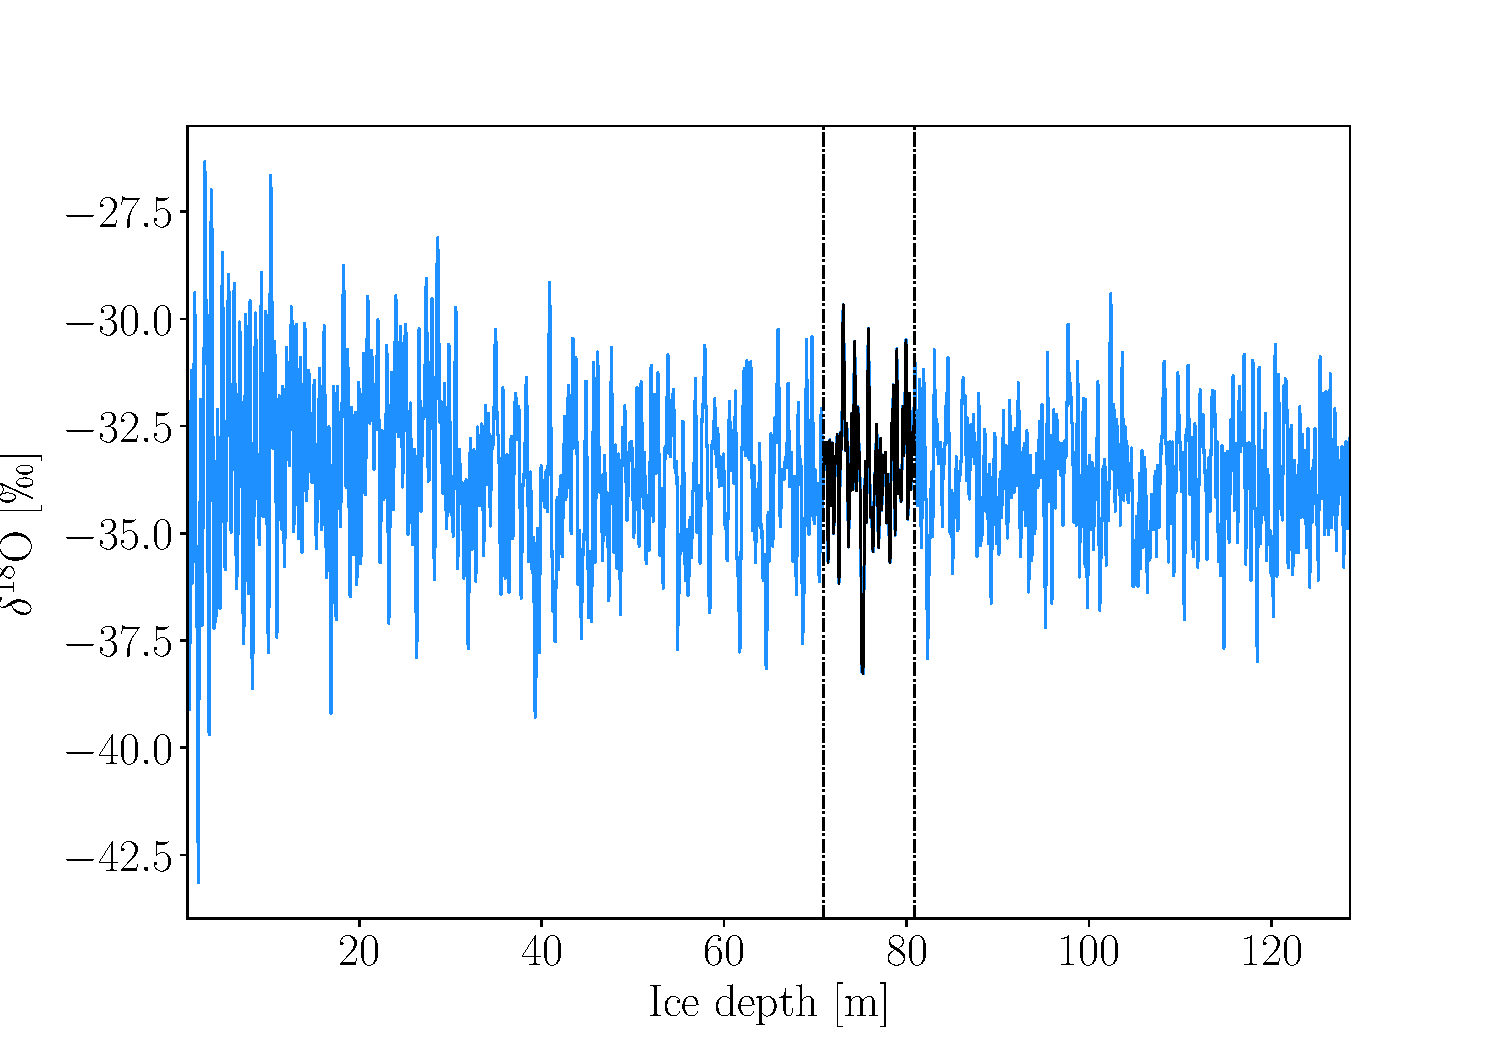
\includegraphics[width=0.9\textwidth]{SiteA_FullIso-eps-converted-to.pdf}
			\caption[Site A isotopes]{Example data from Alphabet Core drilled at site A near Crête.}
			\label{fig:SiteA_FullIso}
		\end{figure}
	}

	\frame{
		\frametitle{Unevenly Sampled Data: Spline Interpolation}
		\begin{figure}
			\centering
			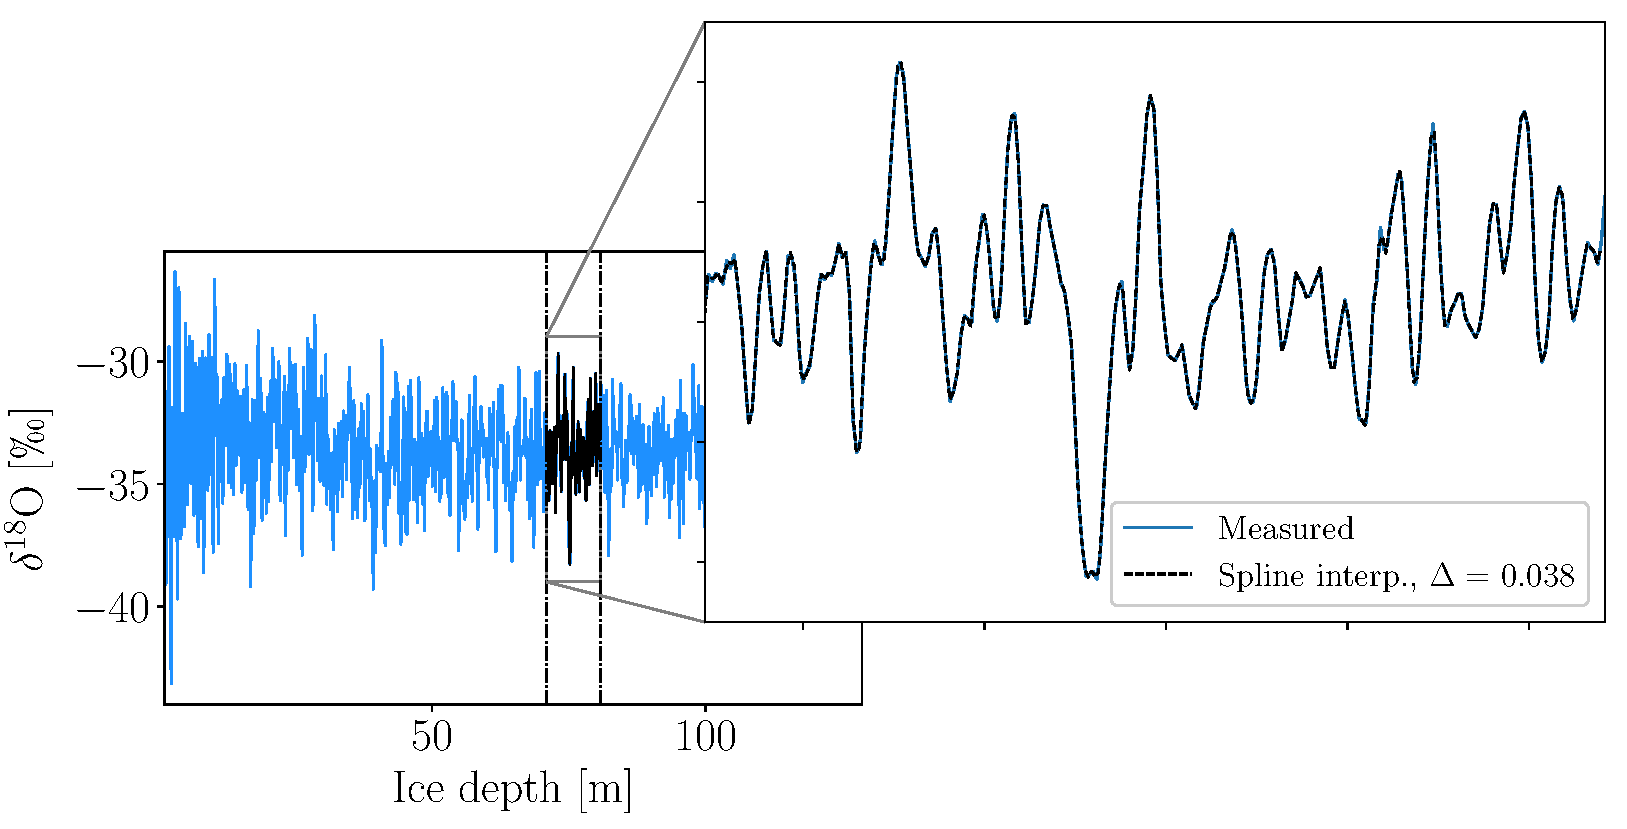
\includegraphics[width=\textwidth]{SiteA_Iso_int_Inset-eps-converted-to.pdf}
			\caption[Site A Laki to Tambora isotopes, w. inset]{Example data from Alphabet Core drilled at site A near Crête. Shows zoom in of data from Laki to Tambora along with spline interpolated data.}
			\label{fig:SiteA_Iso_int_Inset}
		\end{figure}	
		
	}

	\frame{
		\frametitle{Site A}
		
		\begin{figure}
			\centering
			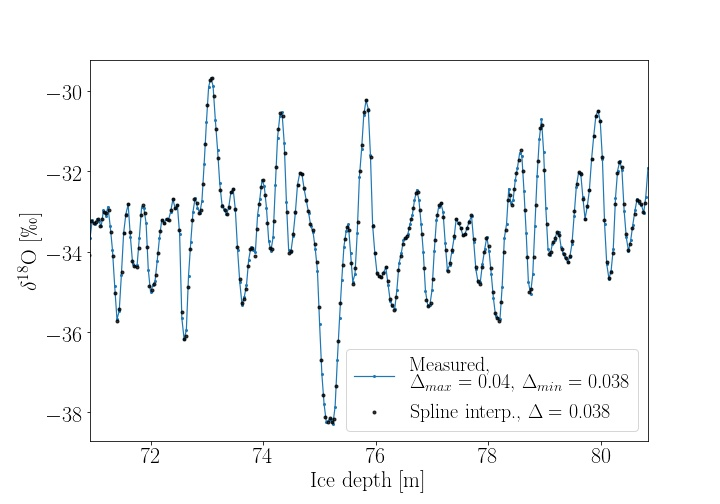
\includegraphics[width=0.9\textwidth]{SiteA_d18OLT_Interp}
			\caption[Site A isotopes]{Site A, raw and cubic spline interpolated data.}
			\label{fig:SiteA_d18OLT_Interp}
		\end{figure}	
	}

	\frame{
		\frametitle{Site G}
		
		\begin{figure}
			\centering
			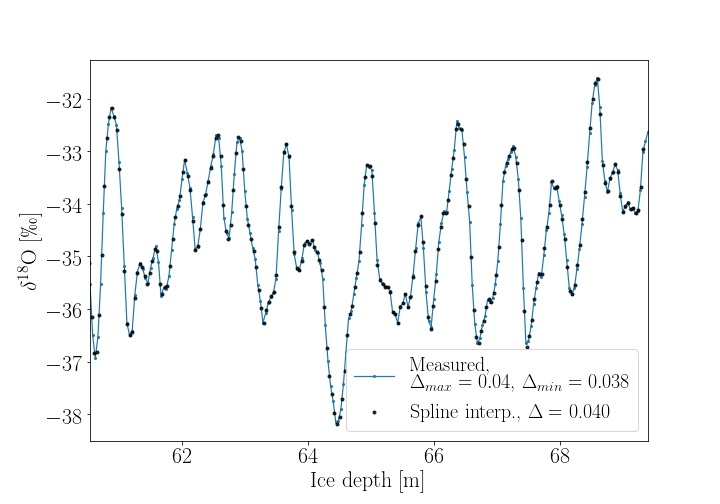
\includegraphics[width=0.9\textwidth]{SiteG_d18OLT_Interp}
			\caption[Site G isotopes]{Site G, raw and cubic spline interpolated data.}
			\label{fig:SiteG_d18OLT_Interp}
		\end{figure}	
	}	



	
		
	\frame{
		\frametitle{Site A: Density and Diffusion Profiles}
		
		\begin{figure}
			\centering
			\begin{subfigure}{.45\textwidth}
				\centering
				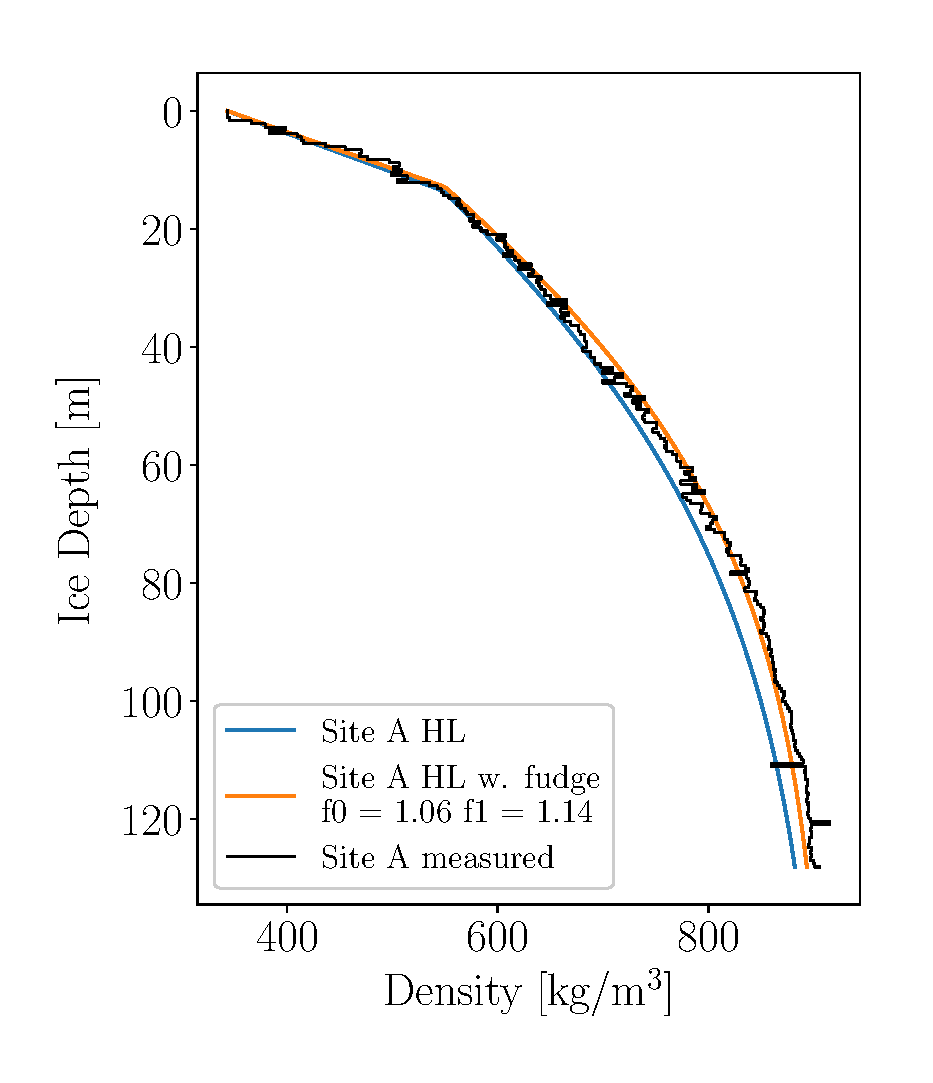
\includegraphics[width=\linewidth]{SiteA_HLdensity.eps}
				\caption[Density-depth profile, Site A]{\tiny Density-depth profiles based on analytical Herron-Langway model. Black is empirical data, blue is purely analytical fit and orange is fudged analytical fit}
				\label{fig:SiteA_HLdensity}
			\end{subfigure}%
			~
			\begin{subfigure}{.45\textwidth}
				\centering
				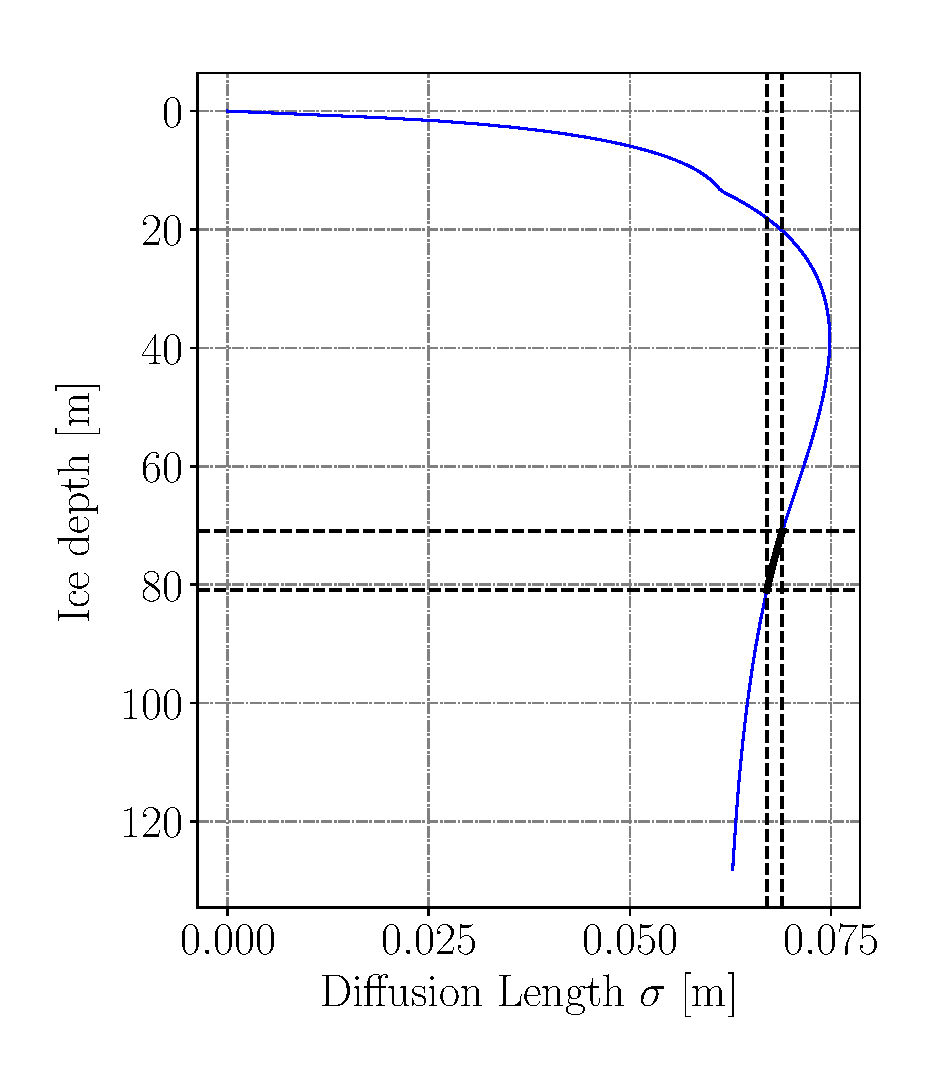
\includegraphics[width=\linewidth]{SiteA_DiffLen.eps}
				\caption[Diffusion length profile, Site A]{\tiny Modeled diffusion length profile based on empirically computed density profile. Black dashed lines indicate ice depth corresponding to date Laki and Tambora eruptions.}
				\label{fig:SiteA_DiffLen}
			\end{subfigure}
			%		\caption{A figure with two subfigures}
			\label{fig:SiteA_CFM}
		\end{figure}
	}
	
	\frame{
		\frametitle{Site G: Density and Diffusion Profiles}
		
		\begin{figure}
			\centering
			\begin{subfigure}{.45\textwidth}
				\centering
				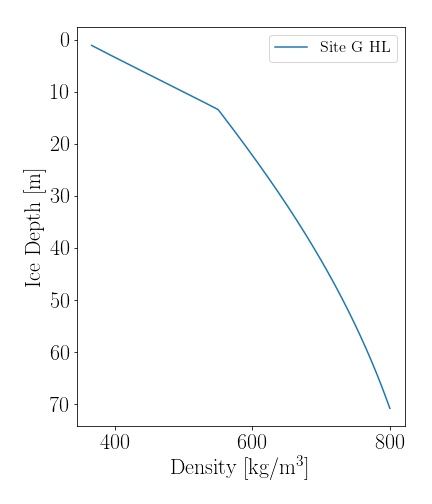
\includegraphics[width=\linewidth]{SiteG_DensProfile_wHL}
				\caption[Density-depth profile, Site G]{\tiny Density-depth profiles based on analytical Herron-Langway model. Black is empirical data, blue is purely analytical fit and orange is fudged analytical fit}
				\label{fig:SiteG_DensProfile_wHL}
			\end{subfigure}%
			~
			\begin{subfigure}{.45\textwidth}
				\centering
				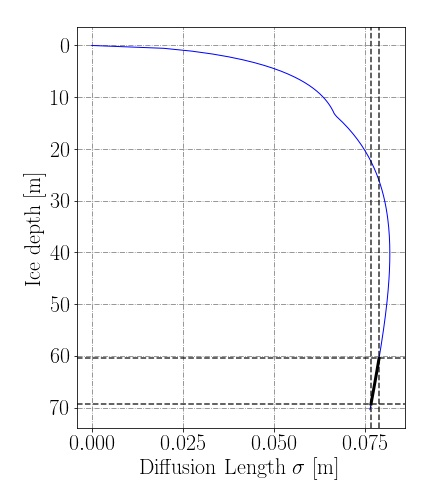
\includegraphics[width=\linewidth]{SiteG_DiffProfile}
				\caption[Diffusion length profile, Site G]{\tiny Modelled diffusion length profile based on empirically computed density profile. Black dashed lines indicate ice depth corresponding to date Laki and Tambora eruptions.}
				\label{fig:SiteG_DiffProfile}
			\end{subfigure}
			%		\caption{A figure with two subfigures}
			\label{fig:SiteG_CFM}
		\end{figure}
	}	
	
	
	
	\subsection{Volcanic Horizons}
	
	\frame{
		\frametitle{Laki and Tambora}
		\begin{itemize}
			\item \textbf{Electrical Conductivity Measurements (ECM)}
			\item \textbf{(Dielectric Profiling (DEP))}
			
		\end{itemize}
		\begin{figure}
			\centering
			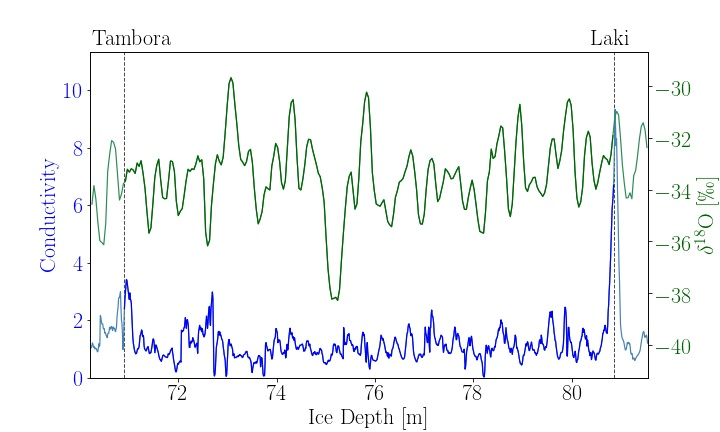
\includegraphics[width=\textwidth]{SiteA_ECMd18O_combo}
			\caption[DEP Laki to Tambora, Site A]{Example of volcanic horizons used for dating of cores, Site A.}
			\label{fig:SiteA_ECMd18O_combo}
		\end{figure}	
	}


	
	\subsection{Back Diffusion}
	
	\begin{frame}  
		\frametitle{Spectral Analysis with DCT}
		\begin{tabular}{cl}  
			\begin{tabular}{c}
				\onslide<1->{
					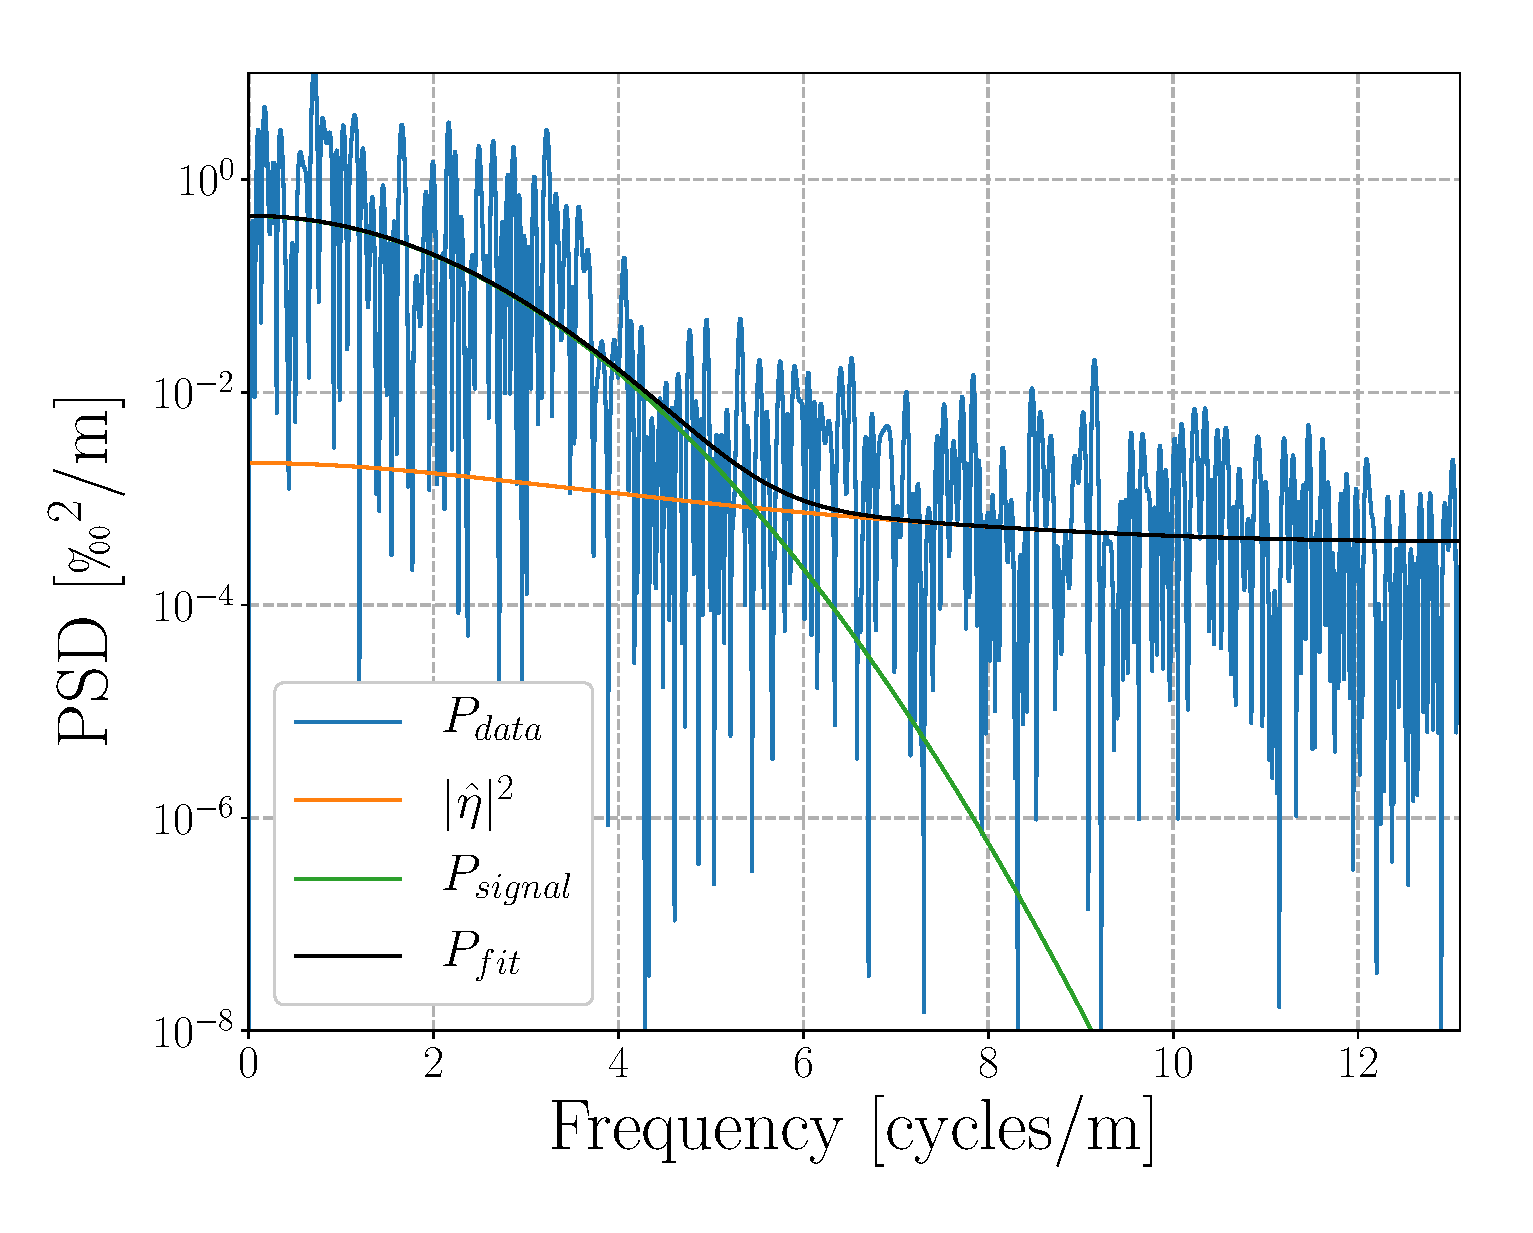
\includegraphics[height=4.5cm, width=5.6cm]{SiteA_PSD.eps}}
			\end{tabular}
			& \begin{tabular}{l}
				\parbox{0.01\linewidth}{\scriptsize %  change the parbox width as appropiate
					\onslide<2-4>{
						\begin{equation*}
							P_{\text{tot}} = P_{\text{signal}} + |\hat{\eta}|^2
					\end{equation*}}
					\onslide<3-4>{
						\begin{equation*}
							|\hat{\eta}|^2 = \frac{\sigma_{\eta}^2\Delta}{|1-a_1 e^{-ik\Delta}|^2}
					\end{equation*}}
					%				\onslide<4>{
					%				\begin{equation*}
					%					P_{\text{signal}} = P_0 e^{-k^2\sigma^2}
					%				\end{equation*}}			
					\onslide<4->{\small
						\begin{equation*}
							P_{\text{signal}} = P_0 e^{-k^2\alert<5>{\sigma^2}}
					\end{equation*}}
				}
				
			\end{tabular}  \\
		\end{tabular}
	\end{frame}
	
	
	\frame{
		\frametitle{Diffusion Lengths and Transfer Functions}
		\onslide<1->{
			\begin{equation}
				\hat{\delta}_{\text{meas}} = \hat{\delta}_{\text{init}}\cdot \hat{M} \Leftrightarrow \hat{\delta}_{\text{init}} = \hat{\delta}_{\text{meas}}\cdot \hat{M}^{-1}
		\end{equation}}
		\onslide<2>{Add an optimal Wiener filter to enhance signal and minimize noise:}
		\onslide<2->{
			\begin{equation}
				\hat{F} = \frac{P_{\text{signal}}}{P_{\text{signal}} + |\hat{\eta}|^2}
		\end{equation}}
		\onslide<3>{yielding a restoration filter as}
		\onslide<3-4>{
			\begin{equation}
				\hat{\delta}_{\text{init}} = \hat{\delta}_{\text{meas}}\cdot \hat{F}\cdot \hat{M}^{-1} = \hat{\delta}_{\text{meas}}\cdot \hat{R}
		\end{equation}}
	}
	
	\frame{
		\frametitle{Filtering}
		
		\begin{figure}
			\centering
			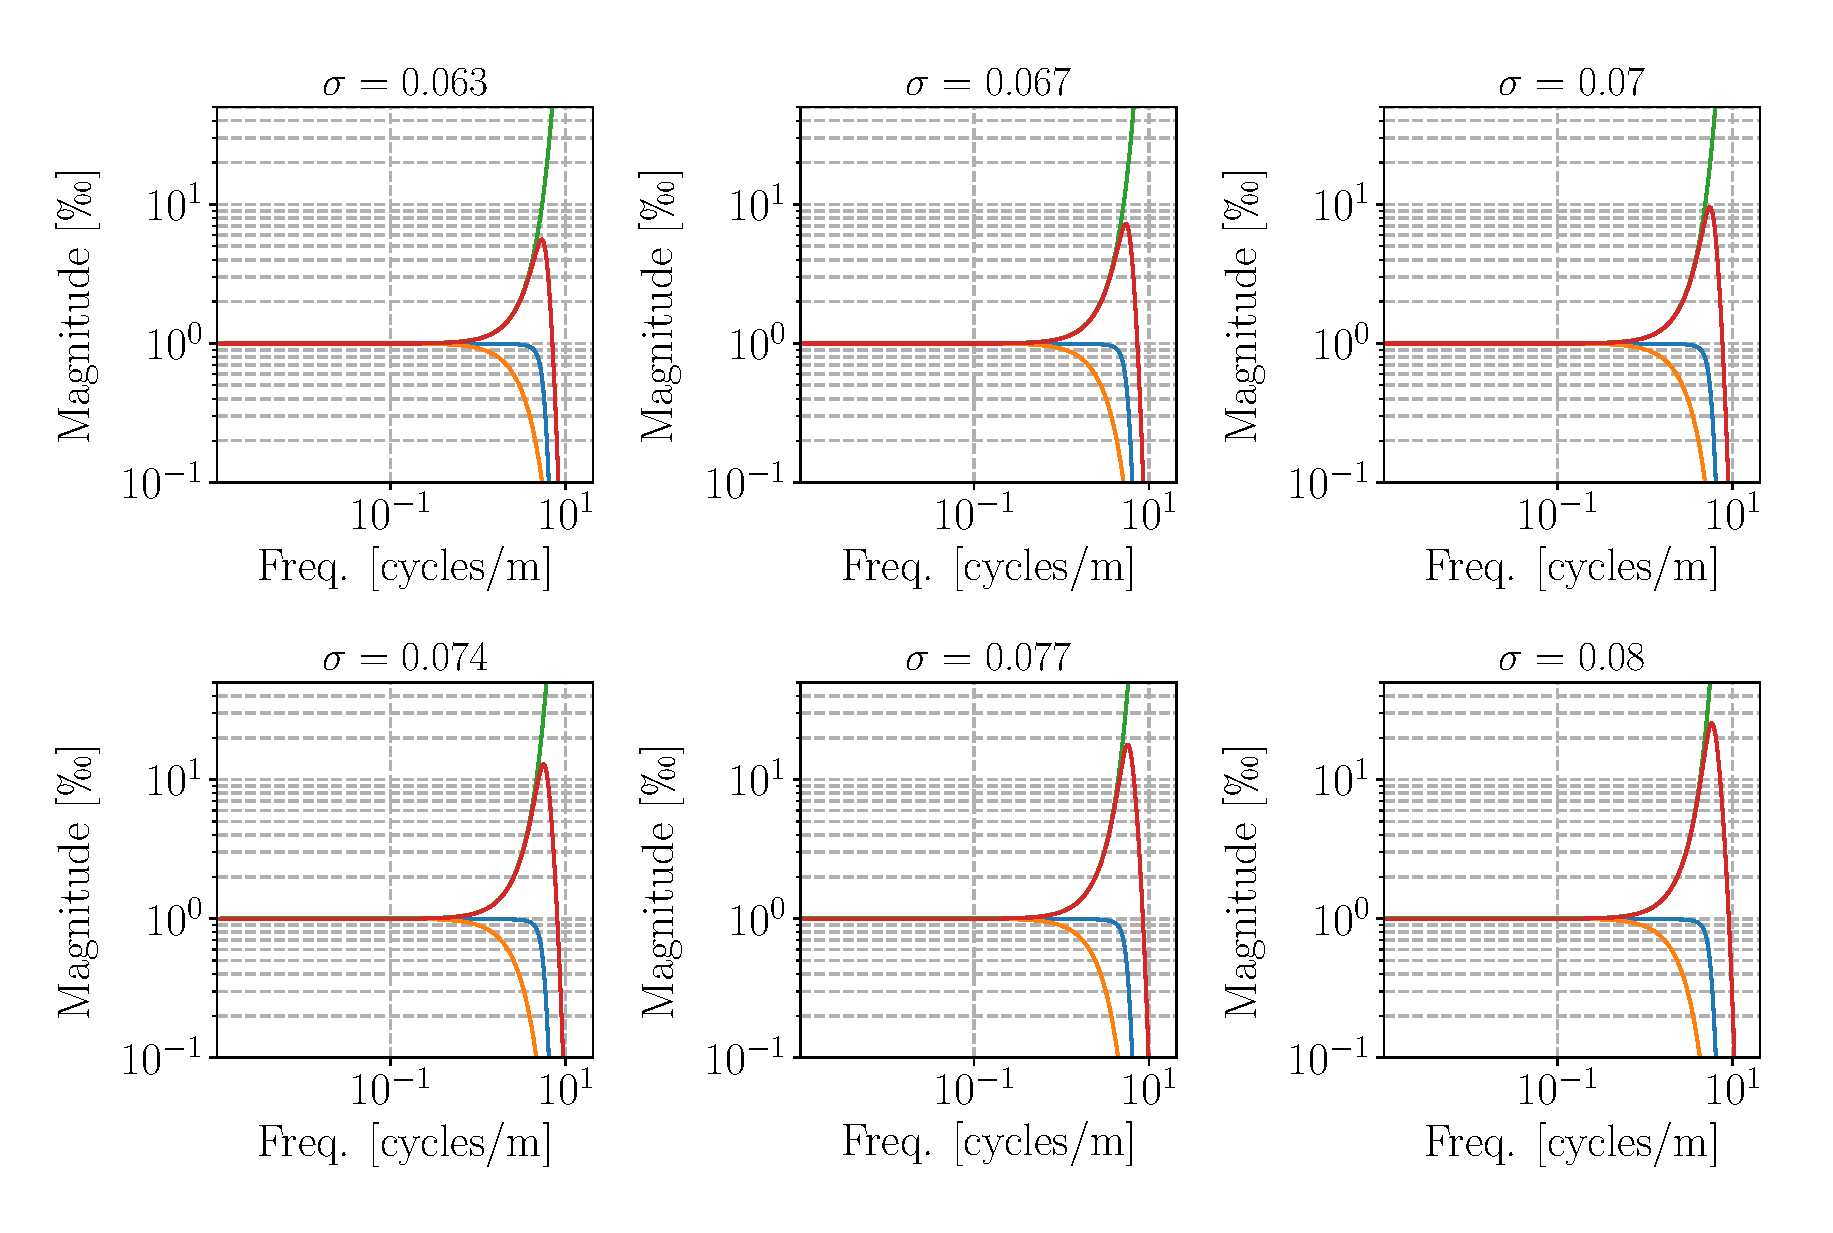
\includegraphics[width=0.9\linewidth]{SiteA_Filters.eps}
			\caption[Filters v. diffusion lengths, Site A]{Frequency filters: The optimal filter found from the PSD (blue), the transfer function (orange), the inverse of the transfer function (green) and the combined signal restoration filter (red).}
			\label{fig:SiteA_Filters}
		\end{figure}
	}
	

	\subsection{}

		
	
	
	\section{Continued Analysis}
	
	
	
	
	\subsection{Peak Detection}
	
	\frame{
		\frametitle{Peak Detection}
		\begin{itemize}
			\item<1-> SciPy.signal.find\_peaks
			\item<2-> N = 32 years btw Tambora and Laki Eruptions
			\item<3-> Best diffusion length estimate algorithm
			\item<4-> Interpolations and resampling 
		\end{itemize}

	}
	
	\frame{
		\frametitle{Diffusion Length Estimate Algorithm}
		\begin{figure}
			\begin{tikzpicture}[node distance=1.5cm, auto,scale=0.7,transform shape]
				\node(start) [startstop] {START};
				%----------------------------------------------------%
				\node(in1) [io, left of=start, xshift=-3.5cm] {Depth series};
				\node(in1pro1) [process, below of=in1, yshift=-0.5cm] {Spline interpolation};
				\node(in1pro2) [process, below of=in1pro1] {Spectral analysis};
				\node(in1pro3) [process, below of=in1pro2] {Wiener filter};
				%	\node(in1pro4) [process, below of=in1pro3] {\textbf{Frequency filters}};	
				
				\draw[arrow] (in1) -- (start);
				\draw[arrow] (start) |- (in1pro1);
				\draw[arrow] (in1pro1) -- (in1pro2);
				\draw[arrow] (in1pro2) -- (in1pro3);
				%	\draw[arrow] (in1pro3) -- (in1pro4);
				
				%----------------------------------------------------%
				\node(in2) [io, right of=start, xshift=3.5cm] {Core specs};
				\node(in2pro1) [process, below of=in2, yshift=-0.5cm] {Density profile};
				\node(in2pro2) [process, below of=in2pro1] {Diffusion profile};
				\node(in2pro3) [process, below of=in2pro2] {$\sigma_0$\textbf{ estimate}};
				
				\draw[arrow] (in2) -- (start);
				\draw[arrow] (start) |- (in2pro1);
				\draw[arrow] (in2pro1) -- (in2pro2);
				\draw[arrow] (in2pro2) -- (in2pro3);
				
				%----------------------------------------------------%
				\node(pro0) [process, below of=start, yshift=-4.5cm] {\textbf{Frequency Filters}};
				\draw[arrow] (in1pro3) -| (pro0);
				\draw[arrow] (in2pro3) -| (pro0);
				\draw[-] (pro0) -- (0,-7);
			\end{tikzpicture}
			\caption[Flowchart 1]{Flowchart of method for diffusion length computation, preliminary analysis steps.}
			\label{Fig:FlowchartDiffLen1}
		\end{figure}
	}

	\frame{
		\frametitle{Diffusion Length Estimate Algorithm}
		\begin{figure}
			\begin{tikzpicture}[node distance=1.5cm, auto,scale=0.5,transform shape]
				\node(pro1) [process, below of=pro0] {\large{\textbf{BACK DIFFUSE}}};
				\node(pro2) [process, below of=pro1] {Count N Peaks};
				\node(dec1) [decision, below of=pro2, yshift=-.5cm] {$N = 32$ ? };
				
				\draw[arrow] (0,-9) -- (pro1);
				\draw[arrow] (pro1) -- (pro2);
				\draw[arrow] (pro2) -- (dec1);
				
				%----------------------------------------------------%	
				\node(pro3a) [process, below of=dec1, xshift=-3cm] {$\sigma = \sigma + \Delta \sigma_1 $};
				\node(pro3apro1) [process, below of=pro3a] {Back diffuse};
				\node(pro3apro2) [process, below of=pro3apro1]  {Count N peaks};
				\node(pro3apro3) [process, below of=pro3apro2, xshift=-2cm] {$\sigma_{\text{final}} = \sigma - 2\cdot\Delta\sigma_1$};
				\node(stop) [startstop, right of=pro3apro3, xshift=2.5cm] {STOP};
				\node(out1) [io, right of=stop, xshift=2.5cm, text width=2.5cm] {\footnotesize{back diffused depth series}};
				\node(out2) [io, below of=out1, text width=1.1cm] {$\sigma_{\text{final}}$};
				
				
				\draw [arrow] (dec1) -| node[anchor=east] {yes} (pro3a);
				\draw [arrow] (pro3a) -- (pro3apro1);
				\draw [arrow] (pro3apro1) -- (pro3apro2);
				\draw [arrow] (pro3apro2) --++ (2,0) node [anchor=west] {If $N$ = 32} |- (pro3a);		
				\draw[arrow] (pro3apro2) --++ (-2,0) node [anchor=east] {If $N > $  32} -| (pro3apro3);
				\draw[arrow] (pro3apro3) -- (stop);
				\draw[arrow] (stop) -- (out1);
				\draw[arrow] (stop) |- (out2);
				
				%----------------------------------------------------%	
				\node(pro3b1) [process, right of=dec1, xshift=3.2cm] {$\sigma = \sigma - \Delta\sigma_2$};
				\node(pro3b2) [process, below of=dec1, xshift=4.7cm] {$\sigma=\sigma+\Delta\sigma_2$};
				
				
				\draw [arrow] (dec1) --(2.45,-13.4) node[anchor=south] {$N > 32$} -- (pro3b1);
				\draw[arrow] (dec1) -- (0,-15) node[anchor=north] {$N < 32$} -- (pro3b2);
				\draw[arrow] (pro3b1) |- (pro1);
				\draw [arrow] (pro3b2) --++ (2,0) |- (pro1);		
				
			\end{tikzpicture}
			\caption[Flowchart 2]{Flowchart of method for diffusion length computation, decision chart.}
			\label{Fig:FlowchartDiffLen2}
		\end{figure}
	}


	\frame{
		\frametitle{Diffusion Length V. Peaks - No Limit}
		\begin{figure}
			\centering
			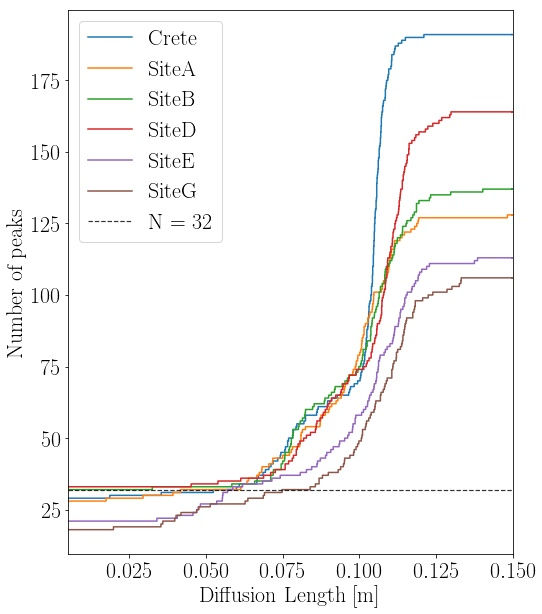
\includegraphics[width=0.5\textwidth]{NpeaksVdiffLen}
			\caption[Diff Len V. Peaks]{Diffusion length used in back diffusion versus counted number of peaks in data series for all cores.}
			\label{fig:NpeaksVdiffLen}
		\end{figure}	
	}
	\frame{
		\frametitle{Diffusion Length V. Peaks - No Limit}
		\begin{figure}
			\centering
			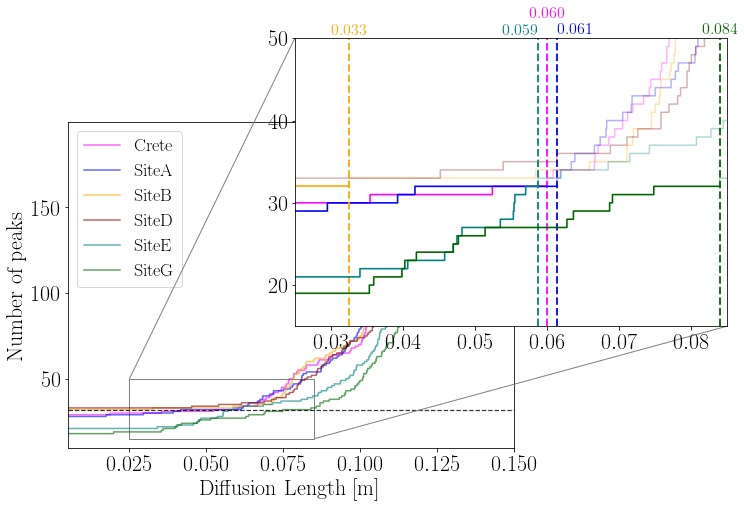
\includegraphics[width=0.9\textwidth]{NpeaksVdiffLen_zoomIn}
			\caption[Diff Len V. Peaks]{Zoom-in around N = 32 peaks and corresponding diffusion length used in back diffusion.}
			\label{fig:NpeaksVdiffLen_zoomIn}
		\end{figure}	
	}


	\frame{
		\frametitle{Cubic Spline Interpolation: Before Deconvolution}
		\begin{figure}
			\centering
			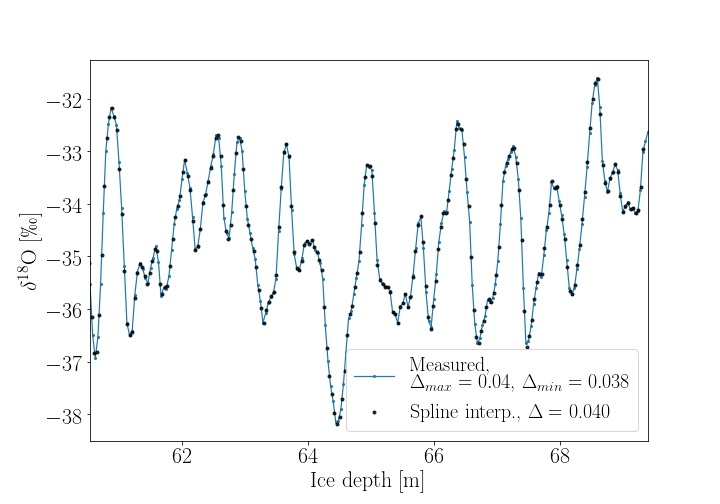
\includegraphics[width=0.9\textwidth]{SiteG_d18OLT_Interp}
			\caption[Interp. BF Deconvolution]{Cubic spline resampling of raw data.}
			\label{fig:SiteG_d18OLT_Interp_BF}
		\end{figure}
	}
	\frame{
		\frametitle{Resampling size V. Diffusion Length Estimate}
		\begin{figure}
			\centering
			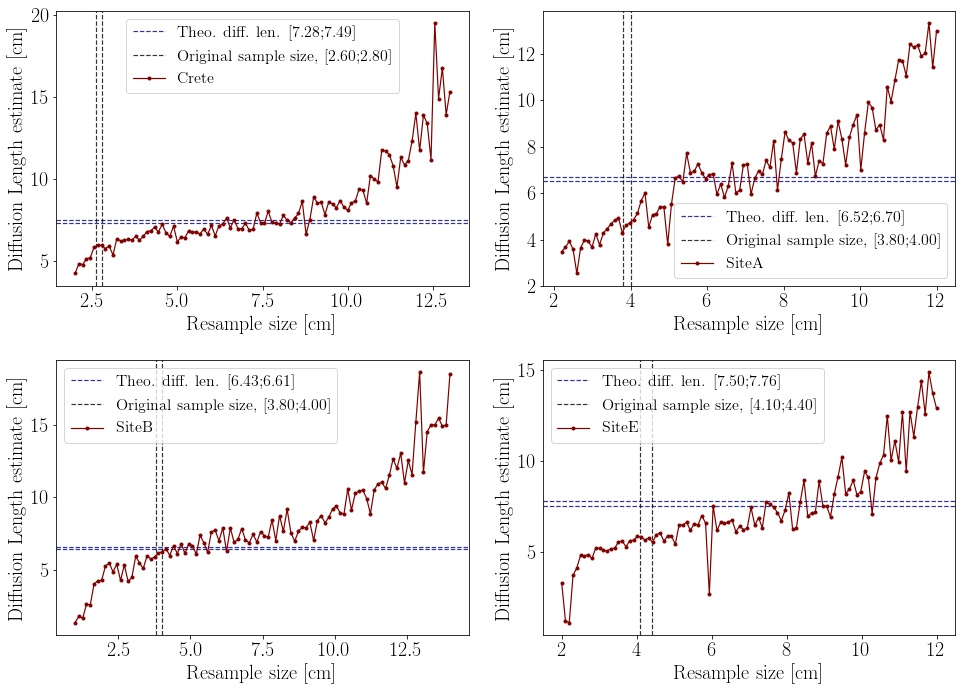
\includegraphics[width=0.9\textwidth]{SamplingVsDiffLen_interpBF}
			\caption[Resampling V. Diff Len, BF]{Resampling size versus diffusion length estimate to result in N = 32 peaks.}
			\label{fig:SamplingVsDiffLen_interpBF}
		\end{figure}
	}


	\frame{
		\frametitle{Cubic Spline Interpolation: After Deconvolution}
		\begin{figure}
			\centering
			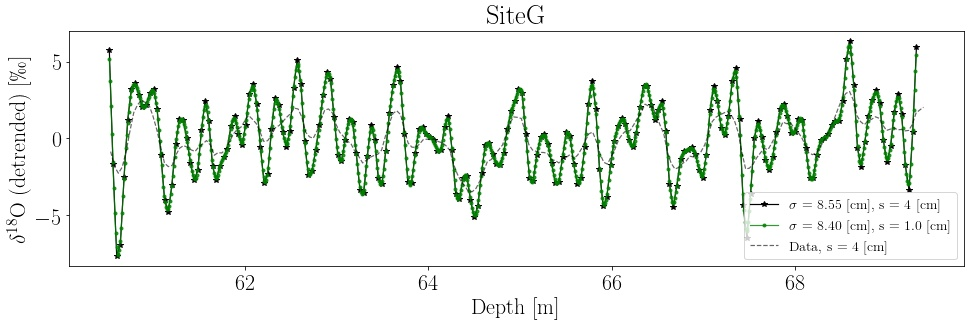
\includegraphics[width=0.9\textwidth]{SiteGResampledAFDecon1cm}
			%\caption[Resampling BF1]{Deconvoluted data with resampling of 9 cm intervals after deconvolution, but before peak finding.}
			\label{fig:SiteAResampledAFDecon1cm}
		\end{figure}
		\begin{figure}
			\centering
			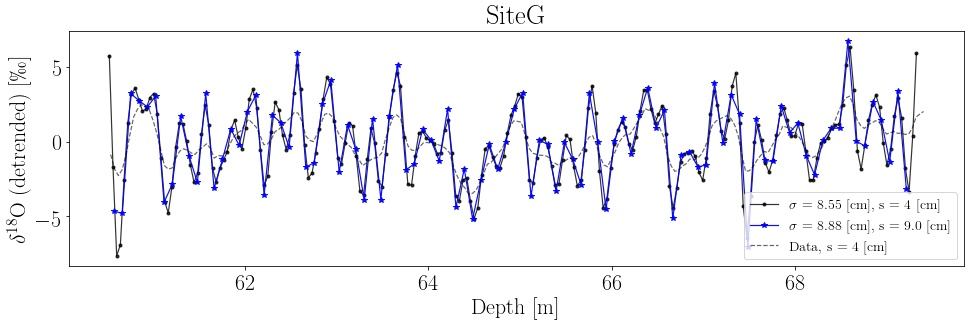
\includegraphics[width=0.9\textwidth]{SiteGResampledAFDecon9cm}
			\caption[Resampling BF9]{Deconvoluted data with resampling of 1 and 9 cm intervals after deconvolution, but before peak finding.}
			\label{fig:SiteAResampledAFDecon9cm}
		\end{figure}
	}
	\frame{
		\frametitle{Resampling size V. Diffusion Length Estimate}
		\begin{figure}
			\centering
			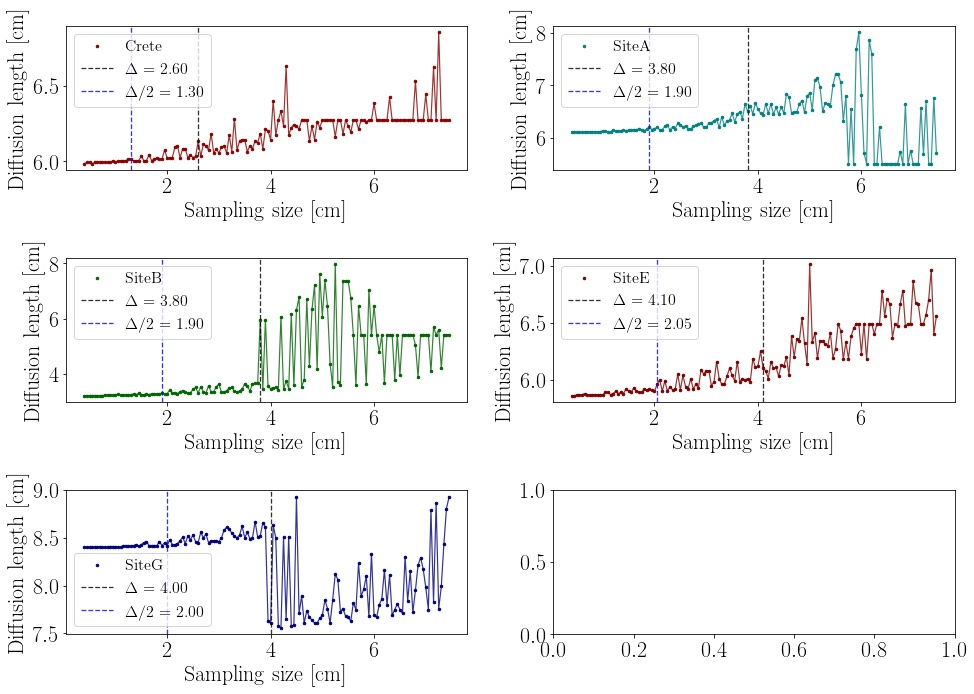
\includegraphics[width=0.9\textwidth]{SamlingVsDiffLen}
			\caption[Resampling V. Diff Len, AF]{Resampling size after deconvolution versus diffusion length estimate to result in N = 32 peaks.}
			\label{fig:SamlingVsDiffLen}
		\end{figure}
	}
	
	\frame{
		\frametitle{Site A: Theoretical V. Estimated Diffusion Length}
		\begin{figure}
			\centering
			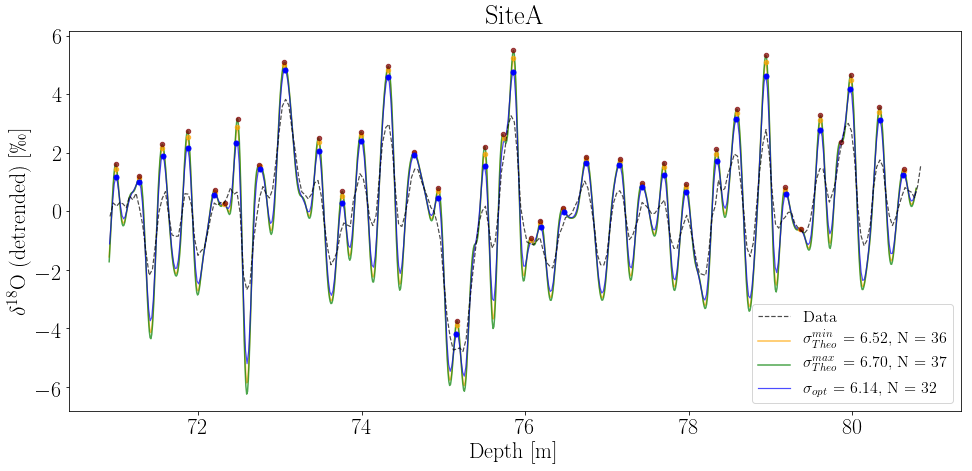
\includegraphics[width=0.9\textwidth]{SiteA_TheoDiffLens}
			\caption[Site A Theo Diff Len]{Data and back diffused signal, using theoretically predicted diffusion lengths and diffusion length estimated through analysis, Site A.}
			\label{fig:SiteA_TheoDiffLens}
		\end{figure}
	}
	\frame{
	\frametitle{Site G: Theoretical V. Estimated Diffusion Length}
	\begin{figure}
		\centering
		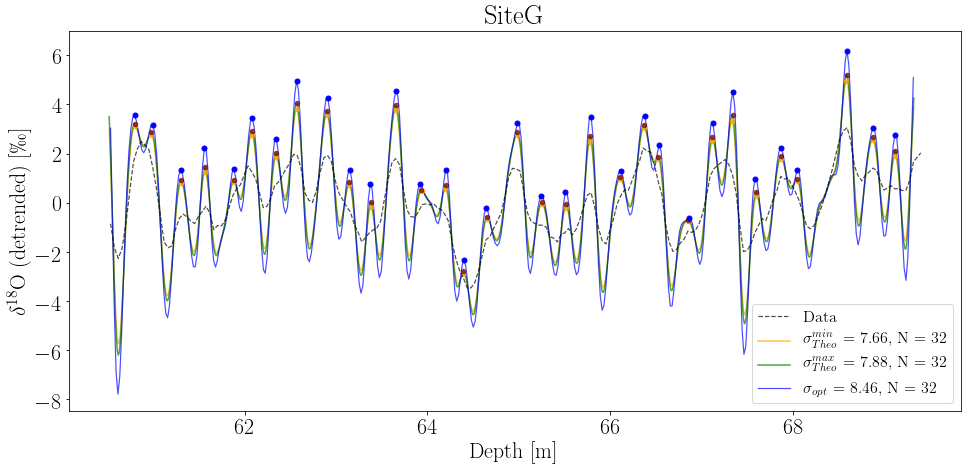
\includegraphics[width=0.9\textwidth]{SiteG_TheoDiffLens}
		\caption[Site G Theo Diff Len]{Data and back diffused signal, using theoretically predicted diffusion lengths and diffusion length estimated through analysis, Site G.}
		\label{fig:SiteG_TheoDiffLens}
	\end{figure}
}


	\frame{
		\frametitle{Diffusion Lengths, All Cores}
		\begin{center}
			\begin{tabular}{l|*{5}{c}}
				& \textbf{Crete} & \textbf{Site A} & \textbf{Site B} & \textbf{Site E} & \textbf{Site G} \\
				\hline
				$\sigma_{Theo}^{min}$ [cm] 	& 7.28 & 6.52 & 6.43 & 7.50 & 7.66 \\
				$\sigma_{Theo}^{max}$ [cm]	& 7.49 & 6.70 & 6.61 & 7.76 & 7.88 \\
				\hline
				\hline
				$\sigma_{est}$ [cm] 		& 6.02 & 6.14 & \begin{tabular}[c]{@{}c@{}}3.27 (N = 32)\\5.85 (N = 33)\end{tabular} & 5.95 & 8.46 \\
%				 & & & 5.85 (N = 33) & & \\
				
			\end{tabular}
		\end{center}

	}

	\subsection{Random Gaps/Missing Data}
	\frame{
		\frametitle{Linear Interpolation, 50 and 100 cm gaps}
		\only<1>{
			\begin{figure}
				\centering
				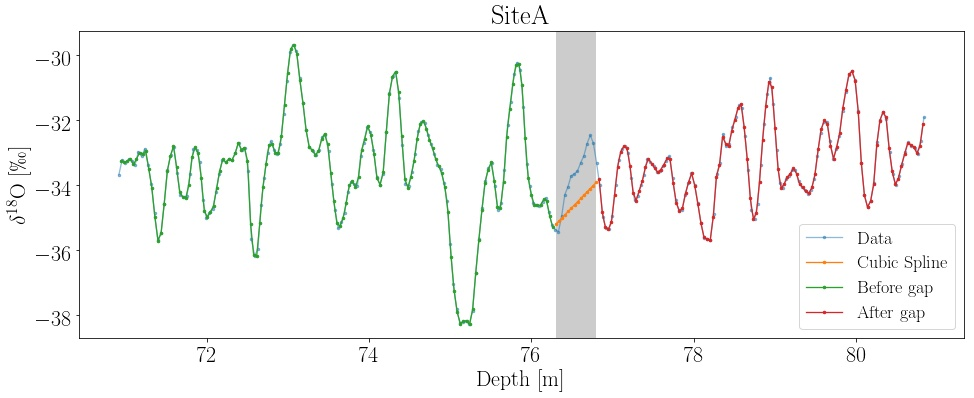
\includegraphics[width=0.8\textwidth]{SiteA_50cmGapWOdecon_Linear}
%				\caption[Site A Theo Diff Len]{}
				\label{fig:SiteA_50cmGapWOdecon_Linear}
			\end{figure}
			\begin{figure}
				\centering
				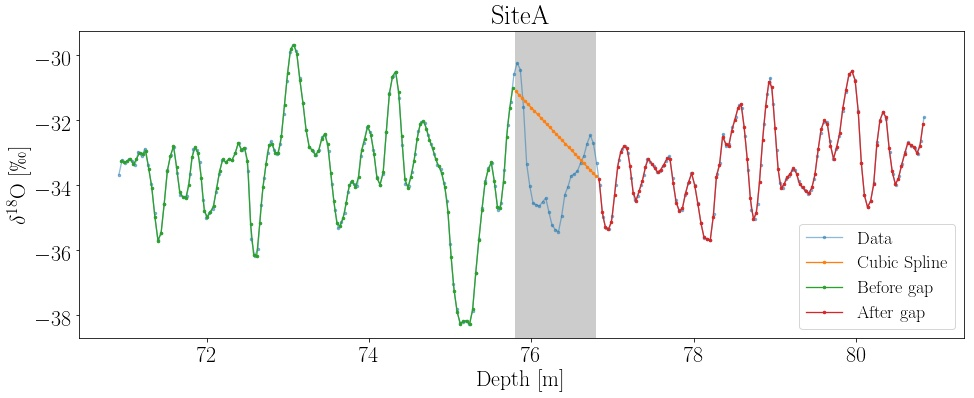
\includegraphics[width=0.8\textwidth]{SiteA_100cmGapWOdecon_Linear}
%				\caption[Site A Theo Diff Len]{}
				\label{fig:SiteA_100cmGapWOdecon_Linear}
			\end{figure}
		
		}
		\only<2>{
			\begin{figure}
				\centering
				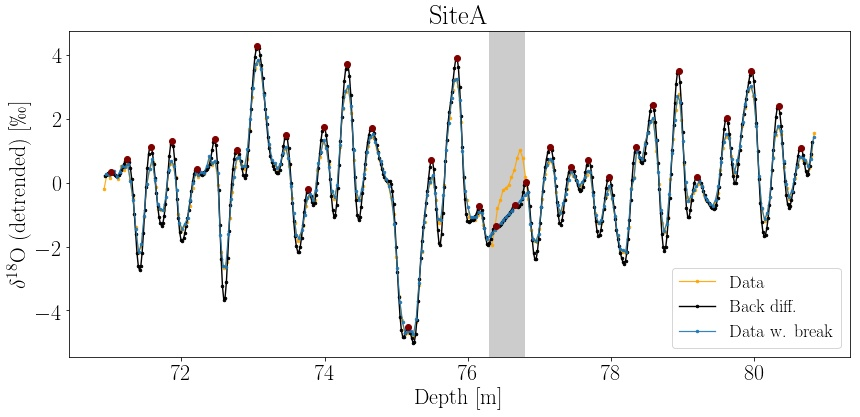
\includegraphics[width=0.7\textwidth]{SiteA_50cmGapWdecon_Linear}
%				\caption[Site A Theo Diff Len]{}
				\label{fig:SiteA_50cmGapWdecon_Linear}
			\end{figure}
			\begin{figure}
				\centering
				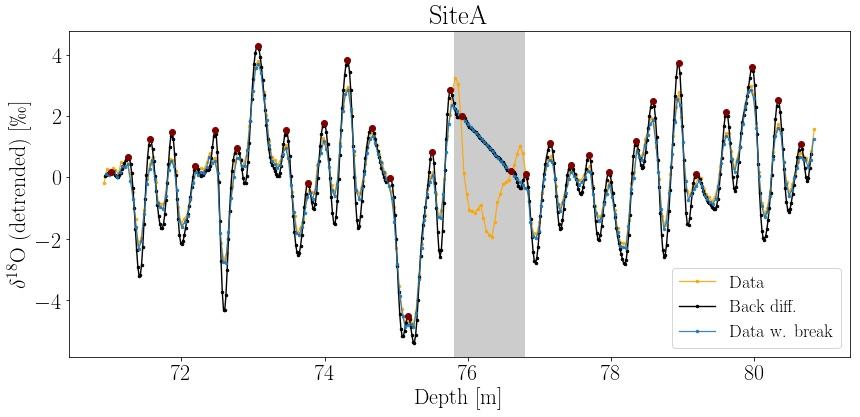
\includegraphics[width=0.7\textwidth]{SiteA_100cmGapWdecon_Linear}
%				\caption[Site A Theo Diff Len]{}
				\label{fig:SiteA_100cmGapWdecon_Linear}
			\end{figure}
			
		}
	}
	\frame{
		\frametitle{Cubic Spline Interpolation}
		\only<1>{
			\begin{figure}
				\centering
				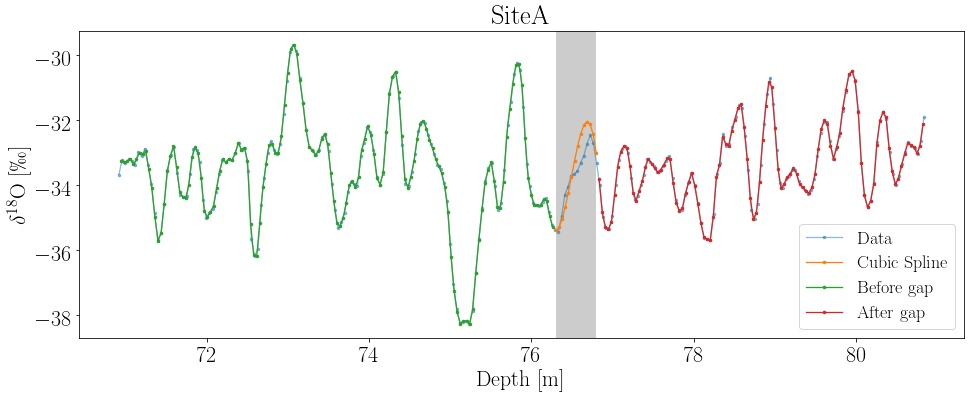
\includegraphics[width=0.8\textwidth]{SiteA_50cmGapWOdecon}
				%				\caption[Site A Theo Diff Len]{}
				\label{fig:SiteA_50cmGapWOdecon}
			\end{figure}
			\begin{figure}
				\centering
				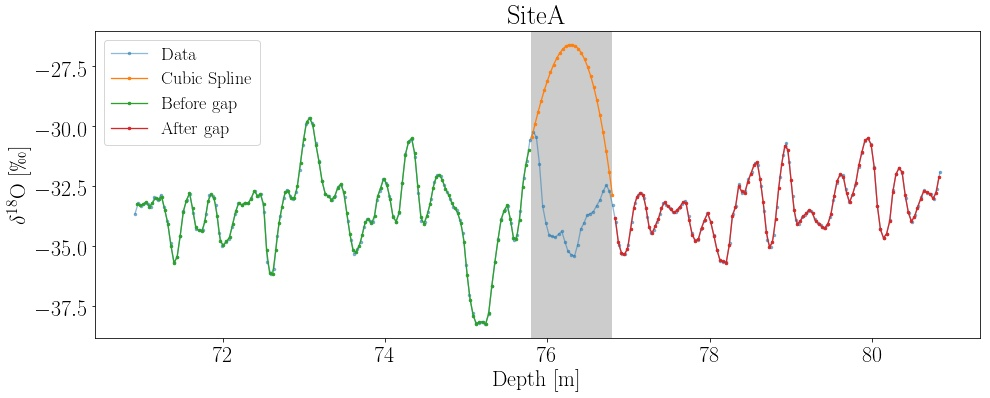
\includegraphics[width=0.8\textwidth]{SiteA_100cmGapWOdecon}
				%				\caption[Site A Theo Diff Len]{}
				\label{fig:SiteA_100cmGapWOdecon}
			\end{figure}
			
		}
		\only<2>{
			\begin{figure}
				\centering
				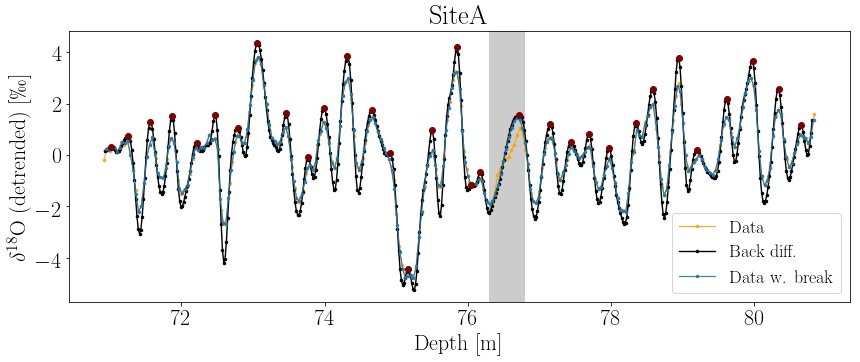
\includegraphics[width=0.8\textwidth]{SiteA_50cmGapWdecon}
				%				\caption[Site A Theo Diff Len]{}
				\label{fig:SiteA_50cmGapWdecon}
			\end{figure}
			\begin{figure}
				\centering
				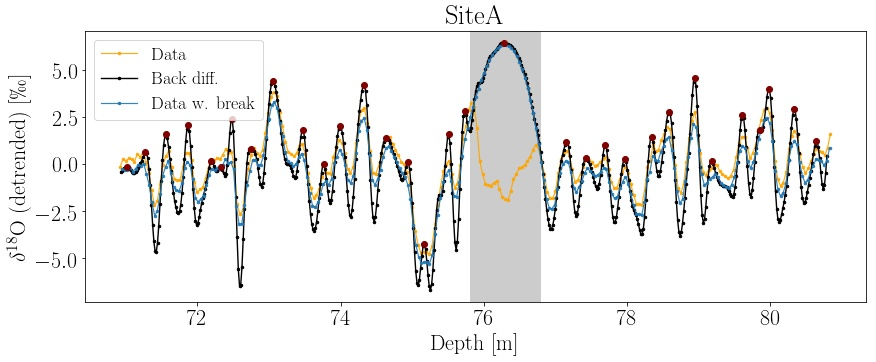
\includegraphics[width=0.8\textwidth]{SiteA_100cmGapWdecon}
				%				\caption[Site A Theo Diff Len]{}
				\label{fig:SiteA_100cmGapWdecon}
			\end{figure}
			
		}
	}
	
	\subsection{Linear Timescale}
	\frame{
		\frametitle{Crete}
		\begin{figure}
			\centering
			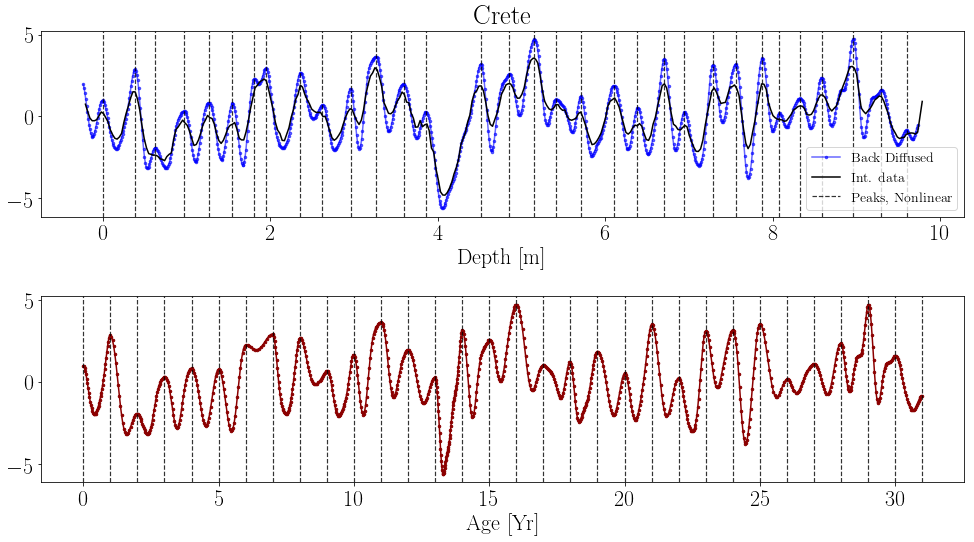
\includegraphics[width=0.9\textwidth]{Crete_LinTimescale}
			\caption[Linear Time Scale, Crete]{Data series on nonlinear and linearized timescales, Crete.}
			\label{fig:Crete_LinTimescale}
		\end{figure}
	}
	\frame{
		\frametitle{Site A}
		\begin{figure}
			\centering
			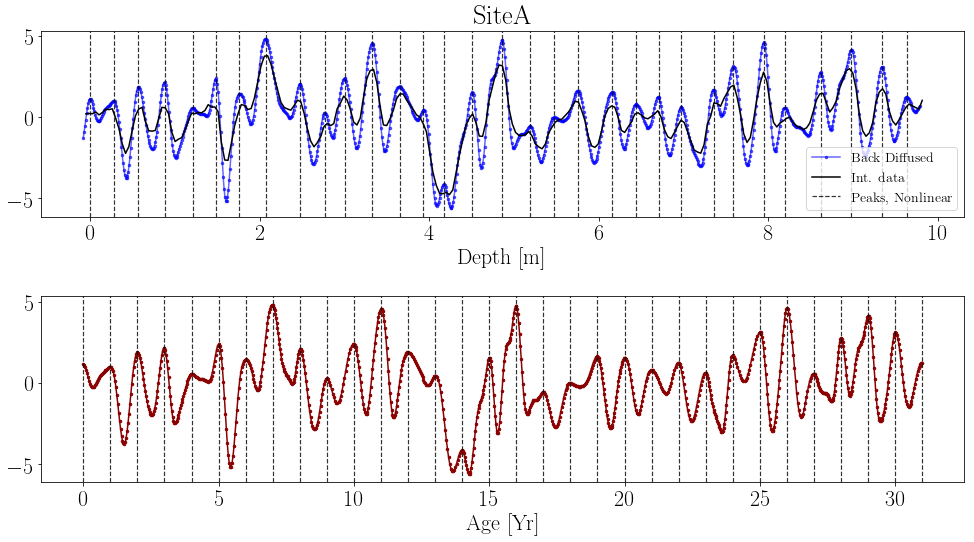
\includegraphics[width=0.9\textwidth]{SiteA_LinTimescale}
			\caption[Linear Time Scale, Site A]{Data series on nonlinear and linearized timescales, Site A.}
			\label{fig:SiteA_LinTimescale}
		\end{figure}
	}
	\frame{
		\frametitle{Site G}
		\begin{figure}
			\centering
			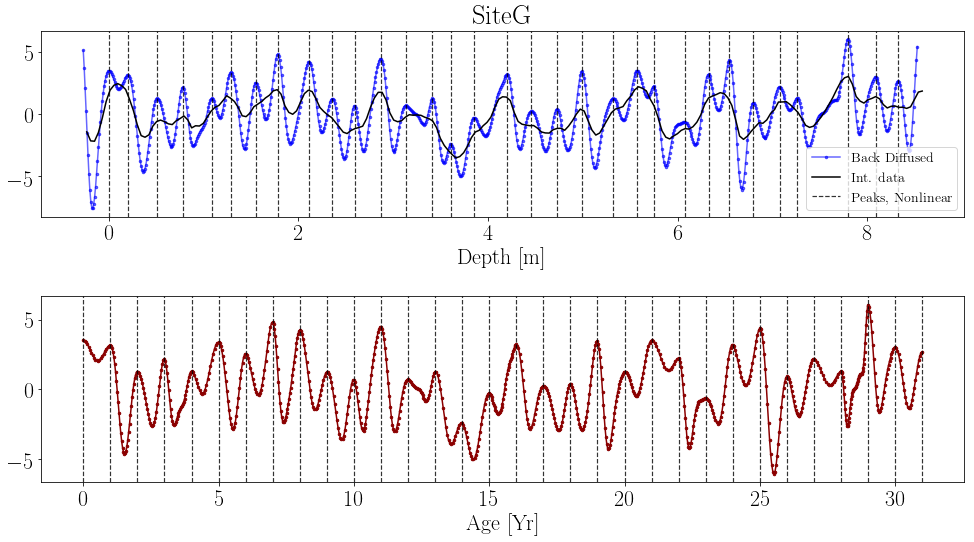
\includegraphics[width=0.9\textwidth]{SiteG_LinTimescale}
			\caption[Linear Time Scale, Site G]{Data series on nonlinear and linearized timescales, Site G.}
			\label{fig:SiteG_LinTimescale}
		\end{figure}
	}
	
	
	\section{Outlook}
		
	
	\frame{
		\frametitle{Further Work}
		\begin{itemize}
			\item Peaks and troughs
			\item Accumulation seasonality
			\item ECM data back diffusion
			\item Missing data reconstruction
			\item Peak/cycle detection through standardization and classification
		\end{itemize}
		
	}
	
	
	\frame{
		\frametitle{Thank you!}
		\LARGE \textbf{Any questions?}
	}
	
	
\appendix

\frame{
	\frametitle{Actual Total Diffusion}
	\onslide<1->{
		Total diffusion in ice and firn
		\begin{equation}
			\sigma_{\text{tot}}(z)^2 = [S(z)\sigma_{\text{firn}}(z)]^2 + \sigma_{\text{ice}}(z)^2
	\end{equation}}
	
	\onslide<2->{Giving an actual measured diffusion length at $z_i$ of
		\begin{equation}
			\sigma(z_i)^2 = \sigma_{\text{firn}}(z_i)^2\,S(z_i) + \sigma_{\text{ice}}(z_i)^2 + \sigma_{\text{dis}}(z_i)^2
		\end{equation}
		with
		\begin{equation}
			\sigma_{\text{dis}}(z_i)^2 = \frac{2\Delta(z_i)^2}{\pi^2}\ln\left(\frac{\pi}{2}\right)
	\end{equation}}
	
}

	\frame{
	\frametitle{Laki and Tambora}
	\begin{itemize}
		\item \textbf{Electrical Conductivity Measurements (ECM)}
		\item \textbf{Dielectric Profiling (DEP)}
	\end{itemize}
	\begin{figure}
		\centering
		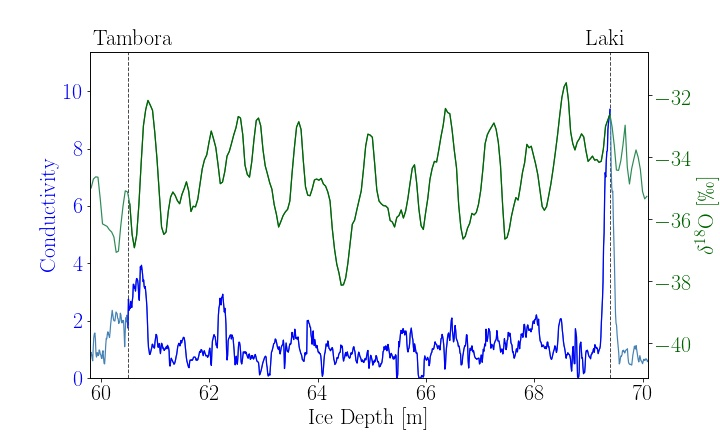
\includegraphics[width=\textwidth]{SiteG_ECMd18O_combo}
		\caption[DEP Laki to Tambora, Site G]{Example of volcanic horizons used for dating of cores, core Site G.}
		\label{fig:SiteG_ECMd18O_combo}
	\end{figure}	
}
	%\begin{frame}[allowframebreaks]
	%\frametitle{References}
	%\begin{multicols}{2}
	%	
	%	\begin{thebibliography}{9}	
	%	\end{thebibliography}
	%\end{multicols}
	%\end{frame}
	%\endgroup
	%    \begin{itemize}[<+->]
	%        \item Something
	%        \item Something more
	%        \item Something third
	%    \end{itemize}
	%    \begin{block}{Definition}
	%        \only<1>{Travel time is the time required by the particle to move from one point to another point.}
	%        \only<2>{Residence time is the time required for the particle to get out of the system.}
	%        \only<3>{Biology is the study of living things.}
	%    \end{block} 
	
	
	
\end{document}


